% ── Εκτεταμένη Περίληψη (Greek extended abstract, NTUA edition) ──

\greekchapter{Εκτεταμένη Περίληψη}

% ══════════════════════════════════════════════════════════════════════════════
\grsection{Εισαγωγή}

\grsubsection{Πλαίσιο και κίνητρο}

Η διάδοση των διασυνδεδεμένων συσκευών στον χώρο της υγείας έχει οδηγήσει στη διαμόρφωση του Διαδικτύου των Ιατρικών Πραγμάτων (Internet of Medical Things, \gls{iomt}): ενός οικοσυστήματος δικτυωμένων ιατρικών οργάνων, φορητών αισθητήρων, συστημάτων παρακολούθησης ασθενών και κλινικών υποδομών που επικοινωνούν μέσω ετερογενών πρωτοκόλλων~\cite{domenech2024ensuring}. Η συνδεσιμότητα αυτή διευρύνει σημαντικά την επιφάνεια επίθεσης. Πολλές ιατρικές συσκευές σχεδιάστηκαν αρχικά για απομονωμένα κλινικά δίκτυα και σήμερα εκτίθενται στις ίδιες απειλές με τα συστήματα γενικής χρήσης, καθώς και σε επιθέσεις που εκμεταλλεύονται αδυναμίες πρωτοκόλλων ειδικών για το νοσοκομειακό περιβάλλον. Οι συνέπειες μιας επιτυχημένης εισβολής δεν περιορίζονται στη διαρροή δεδομένων: όταν παραβιάζονται αντλίες έγχυσης φαρμάκων ή συστήματα παρακολούθησης ζωτικών σημείων, απειλείται άμεσα η ασφάλεια του ασθενούς. Ο Οργανισμός της Ευρωπαϊκής Ένωσης για την Κυβερνοασφάλεια (\gls{enisa}) κατέγραψε σημαντική αύξηση των κυβερνοεπιθέσεων στον τομέα της υγείας την περίοδο 2021--2023, με κυριότερες κατηγορίες το λυτρισμικό, την υποκλοπή δεδομένων και τις επιθέσεις άρνησης υπηρεσίας~\cite{enisa2023health}.

Τα συστήματα ανίχνευσης εισβολών (Intrusion Detection Systems, \gls{ids}) που βασίζονται στη μηχανική μάθηση (\gls{ml}) μαθαίνουν πρότυπα συμπεριφοράς από τη δικτυακή κίνηση και μπορούν να εντοπίσουν τόσο γνωστές όσο και νέες επιθέσεις~\cite{chio2018machine}. Η αποτελεσματικότητά τους, ωστόσο, εξαρτάται καθοριστικά από την ποιότητα, την ποικιλομορφία και την αντιπροσωπευτικότητα των δεδομένων εκπαίδευσης. Τα περισσότερα διαθέσιμα σύνολα δεδομένων \gls{iomt} έχουν αναπτυχθεί ανεξάρτητα, με διαφορετικές τοπολογίες, συσκευές, μεθόδους εξαγωγής χαρακτηριστικών και συμβάσεις ονοματοδοσίας ετικετών. Ως αποτέλεσμα, τα μοντέλα που εκπαιδεύονται σε ένα μόνο σύνολο αποδίδουν καλά στις συνθήκες του, αλλά αποτυγχάνουν όταν εφαρμόζονται σε διαφορετικό περιβάλλον~\cite{domenech2025evaluating}.

\grsubsection{Διατύπωση του προβλήματος}

Η ανάπτυξη εύρωστων και γενικεύσιμων μοντέλων \gls{ids} για περιβάλλοντα \gls{iomt} παρεμποδίζεται από τέσσερα αλληλένδετα προβλήματα:
\begin{enumerate}[leftmargin=*, label=\textbf{Π\arabic*.}, nosep]
  \item \textbf{Απομόνωση των συνόλων δεδομένων.} Τα CICIoMT2024~\cite{dadkhah2024ciciomt} και IoMT-TrafficData~\cite{areia2024iomt} καλύπτουν το καθένα ένα περιορισμένο υποσύνολο επιθέσεων, πρωτοκόλλων και συμπεριφορών συσκευών· κανένα δεν καλύπτει πλήρως το τοπίο απειλών.
  \item \textbf{Ετερογένεια χαρακτηριστικών.} Διαφορετικά εργαλεία εξαγωγής (π.χ.\ CICFlowMeter έναντι Zeek) παράγουν δομικά ασύμβατους χώρους χαρακτηριστικών, οπότε η απευθείας συνένωση είναι αδύνατη.
  \item \textbf{Ασυνέπεια ετικετών.} Η ίδια επίθεση ονομάζεται διαφορετικά σε κάθε σύνολο (π.χ.\ \textit{DDoS\_TCP\_Flood} έναντι \textit{DoS}), γεγονός που αποκλείει την από κοινού εκπαίδευση και αξιολόγηση.
  \item \textbf{Υπερπροσαρμογή σε ένα πεδίο.} Τα μοντέλα μίας πηγής μαθαίνουν τις ιδιαιτερότητες του συγκεκριμένου δικτύου και εμφανίζουν χαμηλά ποσοστά ανίχνευσης σε κίνηση από άλλα περιβάλλοντα.
\end{enumerate}

\grsubsection{Ερευνητικό ερώτημα και στόχοι}

Η εργασία καθοδηγείται από το κεντρικό ερευνητικό ερώτημα: \textit{Πώς μπορεί η ενοποίηση πολλαπλών ετερογενών συνόλων δεδομένων να βελτιώσει την απόδοση και τη γενικευσιμότητα ενός μοντέλου μηχανικής μάθησης στην ανίχνευση εισβολών σε περιβάλλοντα IoMT;} Για την απάντησή του τέθηκαν έξι στόχοι: (Σ1) συλλογή και διερευνητική ανάλυση των συνόλων δεδομένων· (Σ2) τυποποιημένη εξαγωγή χαρακτηριστικών με το εργαλείο MIOTTA-NPT~\cite{leon2025miotta}· (Σ3) σχεδιασμός και εκτέλεση ροής ενοποίησης με εναρμόνιση ετικετών, διασφάλιση ποιότητας, κανονικοποίηση και ιχνηλάτηση προέλευσης· (Σ4) επικύρωση της ακεραιότητας του ενοποιημένου συνόλου· (Σ5) υποδομή για αυστηρή αξιολόγηση μεταξύ πεδίων (cross-domain)· και (Σ6) ανάπτυξη και αξιολόγηση μοντέλων \gls{ids}, συμπεριλαμβανομένης της εφαρμογής τους σε πραγματική νοσοκομειακή κίνηση (HospNet26~\cite{hospnet26}).

\grsubsection{Συνεισφορές}

Οι κύριες συνεισφορές της εργασίας είναι: (α)~μια αναπαραγώγιμη μεθοδολογία ενοποίησης σε επίπεδο ακατέργαστων καταγραφών πακέτων (\gls{pcap}), η οποία παρήγαγε ένα ενιαίο σύνολο 8.011.534 εγγραφών, δημόσια διαθέσιμο με DOI \href{https://doi.org/10.34810/DATA3305}{10.34810/DATA3305}~\cite{unified_iomt_csuc2026}· (β)~εμπειρική τεκμηρίωση ότι η ενοποίηση βελτιώνει δραστικά τη γενίκευση· (γ)~ένα πλαίσιο αξιολόγησης μεταξύ πεδίων βασισμένο στην καταγραφή προέλευσης· (δ)~η πρώτη ποσοτική μέτρηση του χάσματος «εργαστηρίου--κλινικής» σε πραγματική νοσοκομειακή κίνηση· και (ε)~στατιστική επικύρωση με τον έλεγχο McNemar. Τα κύρια ευρήματα έγιναν δεκτά για δημοσίευση ως πλήρες άρθρο στο \textit{Workshop on Cybersecurity in Healthcare Operations (SecHealth)}, στο πλαίσιο του διεθνούς συνεδρίου ARES~2026.

% ══════════════════════════════════════════════════════════════════════════════
\grsection{Υπόβαθρο και σχετικές εργασίες}

\grsubsection{Ασφάλεια IoMT και ανίχνευση εισβολών}

Τα περιβάλλοντα \gls{iomt} χαρακτηρίζονται από αυστηρές απαιτήσεις αξιοπιστίας, καθυστέρησης και εμπιστευτικότητας~\cite{dimitrov2016medical}. Η πρόκληση ασφάλειας ενισχύεται από τους περιορισμένους υπολογιστικούς πόρους των συσκευών, τη συνύπαρξη πολλαπλών πρωτοκόλλων (Wi-Fi, \gls{ble}, \gls{mqtt}, \gls{coap}, ZigBee), τον μακρύ κύκλο ζωής παλαιών συστημάτων χωρίς ενημερώσεις και, κυρίως, τις άμεσες επιπτώσεις στην ασφάλεια των ασθενών. Τα \gls{ids} ταξινομούνται ως προς την πηγή δεδομένων σε δικτυακά (\gls{nids}) και σε συστήματα υπολογιστή-ξενιστή (\gls{hids}), και ως προς τη μέθοδο ανίχνευσης σε συστήματα βασισμένα σε υπογραφές (\gls{sids}) και σε ανωμαλίες (\gls{aids})~\cite{khraisat2019survey}. Για το \gls{iomt}, ο συνδυασμός δικτυακής ανάπτυξης και ανίχνευσης ανωμαλιών θεωρείται ο πλέον βιώσιμος, διότι δεν απαιτεί παρεμβάσεις στις ίδιες τις ιατρικές συσκευές~\cite{domenech2024ensuring, weber2023attack}. Οι κλασικοί αλγόριθμοι \gls{ml} (\gls{dt}, \gls{rf}, \gls{xgb}) πλεονεκτούν σε χαμηλό υπολογιστικό κόστος και ερμηνευσιμότητα~\cite{heidari2023iot}, ενώ οι προσεγγίσεις βαθιάς μάθησης μαθαίνουν ιεραρχικές αναπαραστάσεις απευθείας από τα δεδομένα~\cite{lopez2025nprint}.

\grsubsection{Σύνολα δεδομένων}

Ο Πίνακας~\ref{gr:tab:datasets} συνοψίζει τα τρία σύνολα δεδομένων της εργασίας. Τα δύο σύνολα εκπαίδευσης χρησιμοποιούν δομικά ασύμβατες μεθόδους εξαγωγής χαρακτηριστικών (CIC έναντι Zeek), ενώ το HospNet26 είναι ήδη διαθέσιμο στη μορφή του MIOTTA-NPT και μοιράζεται τον ίδιο χώρο 58 χαρακτηριστικών με τα επανεπεξεργασμένα σύνολα εκπαίδευσης.

\begin{table}[!htbp]
\centering
\caption[]{Συγκριτική σύνοψη των συνόλων δεδομένων της εργασίας.}
\label{gr:tab:datasets}
\small
\begin{tabularx}{\textwidth}{@{}l X X X@{}}
\toprule
\textbf{Χαρακτηριστικό} & \textbf{CICIoMT2024} & \textbf{IoMT-TrafficData} & \textbf{HospNet26} \\
\midrule
Ρόλος & Εκπαίδευση / έλεγχος & Εκπαίδευση / έλεγχος & Δοκιμή γενίκευσης \\
Πεδίο & Πειραματική διάταξη IoMT & Πειραματική διάταξη IoMT & Πραγματικό νοσοκομείο \\
Έτος & 2024 & 2024 & 2026 \\
Συσκευές & 40 (πραγματικές + εξομοιωμένες) & Πραγματικές + προσομοιωμένες & Παραγωγικό κλινικό δίκτυο \\
Τύποι επιθέσεων & 18 & 6 κατηγορίες & Καμία (μόνο καλόβουλη) \\
Αρχικά χαρακτηριστικά & 45 & 101 (Zeek) & -- \\
Εργαλείο εξαγωγής & CIC (εσωτερικό) & Zeek & MIOTTA-NPT \\
Διαθέσιμα PCAP & Ναι & Ναι & Ναι \\
\bottomrule
\end{tabularx}
\end{table}

\grsubsection{Το εργαλείο MIOTTA-NPT}

Το MIOTTA-NPT~\cite{leon2025miotta, miotta_npt_github} είναι ένα παραμετροποιήσιμο εργαλείο ανοικτού κώδικα, ανεπτυγμένο από ερευνητική ομάδα του UPC, που μετατρέπει αρχεία \gls{pcap} σε δομημένα σύνολα δεδομένων. Υποστηρίζει έξοδο CSV με στατιστικά χαρακτηριστικά ή δυαδικές αναπαραστάσεις nPrint~\cite{holland2021nprint}, καθώς και τέσσερις τρόπους συνάθροισης (πακέτο, ροή, παράθυρο, συνδυασμένο). Στον \textit{συνδυασμένο} τρόπο εξάγει έως 103 χαρακτηριστικά: μεταδεδομένα σύνδεσης, στατιστικά μεγέθους πακέτων, κατευθυντικές μετρικές, κατανομές σημαιών \gls{tcp}, χρόνους μεταξύ αφίξεων (\gls{iat}) και δυναμικά μεγέθη ροής. Το καθοριστικό πλεονέκτημα για την ενοποίηση είναι ότι, επεξεργαζόμενο τις ακατέργαστες καταγραφές κάθε συνόλου με την ίδια διαμόρφωση, παράγει \textit{ταυτόσημους} χώρους χαρακτηριστικών, επιλύοντας την ετερογένεια στην πηγή αντί για εκ των υστέρων αντιστοίχιση.

\grsubsection{Προσεγγίσεις ενοποίησης και ερευνητικά κενά}

Η βιβλιογραφία δείχνει ότι ο έλεγχος μεταξύ διαφορετικών συνόλων αποκαλύπτει απώλειες έως και 30 ποσοστιαίων μονάδων στο macro-F1~\cite{abouhouran2025federated}. Οι προσεγγίσεις ενοποίησης περιλαμβάνουν γενικά μοντέλα ενοποίησης δεδομένων (GUDM~\cite{ali2015gudm}), επανεξαγωγή από αρχεία \gls{pcap} (UM-NIDS/META~\cite{khan2024umnids}, Nxcap~\cite{noblet2025nxcap}), σημασιολογική αντιστοίχιση χαρακτηριστικών και εναρμόνιση ετικετών σε ομοσπονδιακή μάθηση~\cite{abouhouran2025federated}. Η εργασία υιοθετεί μια \textit{υβριδική} στρατηγική: επανεξαγωγή σε επίπεδο \gls{pcap} με το MIOTTA-NPT, εναρμόνιση ετικετών πολλαπλών επιπέδων, διασφάλιση ποιότητας και ιχνηλάτηση προέλευσης. Τα κενά που καλύπτει είναι: (i)~δεν υπήρχε ενοποίηση των CICIoMT2024 και IoMT-TrafficData σε επίπεδο \gls{pcap}· (ii)~κανένα \gls{ids} για \gls{iomt} δεν είχε αξιολογηθεί σε πραγματική νοσοκομειακή κίνηση· και (iii)~δεν υπήρχε ενιαίο, έτοιμο για \gls{ml} σύνολο με εναρμονισμένες ετικέτες και ελεγχόμενη προέλευση.

% ══════════════════════════════════════════════════════════════════════════════
\grsection{Σχεδιασμός της μεθοδολογίας ενοποίησης}

Η στρατηγική ενοποίησης οργανώνεται ως ροή πολλαπλών σταδίων (Σχήμα~\ref{gr:fig:pipeline}) και διέπεται από πέντε αρχές: τυποποίηση στην πηγή, εναρμόνιση ετικετών, διατήρηση της προέλευσης, ενσωμάτωση της ποιότητας ως βασικού σταδίου και επεκτασιμότητα σε νέα σύνολα δεδομένων (π.χ.\ από την υπό ανάπτυξη πειραματική διάταξη MIoTTA-UPC).

\begin{figure}[!htbp]
\centering
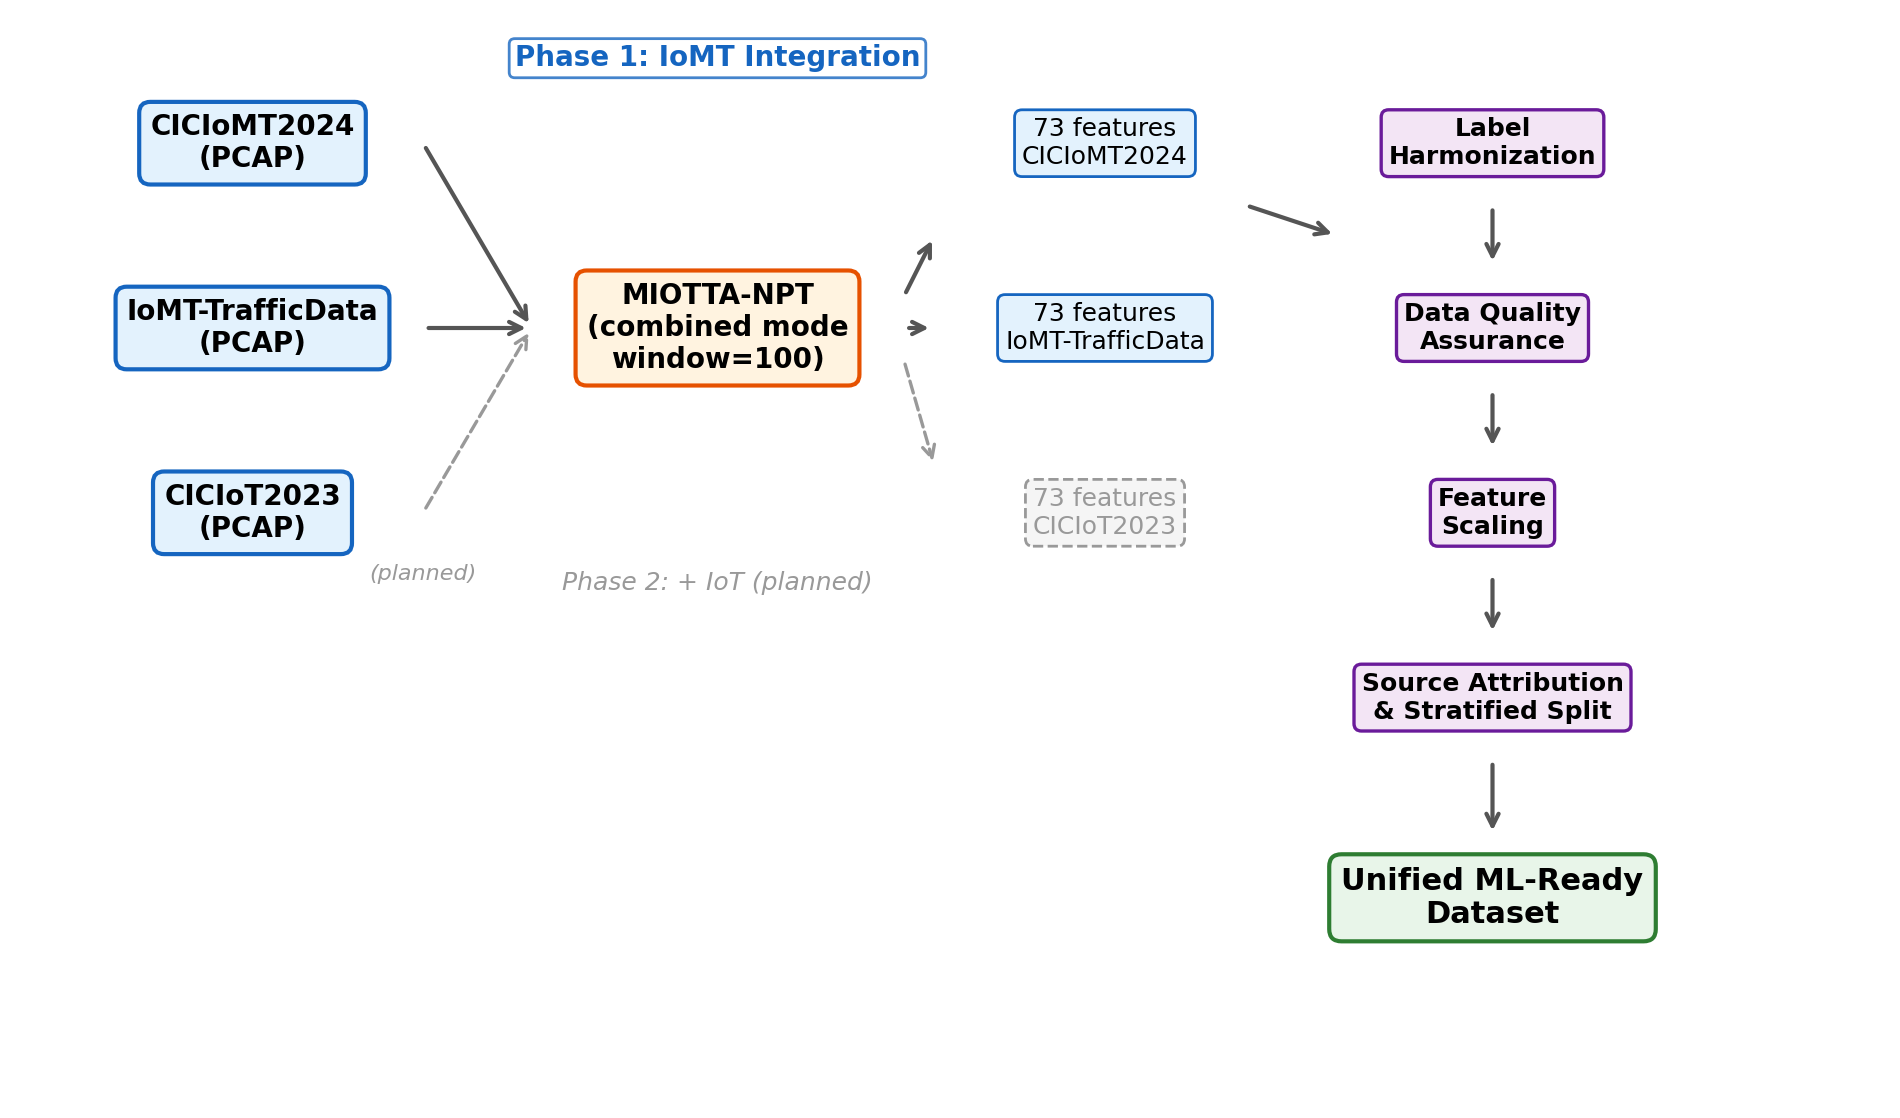
\includegraphics[width=\textwidth]{pipeline_overview.png}
\caption[]{Επισκόπηση της ροής ενοποίησης πολλαπλών σταδίων. Οι ακατέργαστες καταγραφές πακέτων των CICIoMT2024 και IoMT-TrafficData επεξεργάζονται από το MIOTTA-NPT με ταυτόσημη διαμόρφωση και στη συνέχεια περνούν από εναρμόνιση ετικετών, διασφάλιση ποιότητας, κανονικοποίηση και στρωματοποιημένο διαχωρισμό, παράγοντας το τελικό ενοποιημένο σύνολο.}
\label{gr:fig:pipeline}
\end{figure}

\grsubsection{Τυποποιημένη εξαγωγή χαρακτηριστικών}

Όλα τα σύνολα επεξεργάζονται με το MIOTTA-NPT στον συνδυασμένο τρόπο (ροή και παράθυρο) με μέγεθος παραθύρου 100 πακέτων, που εξασφαλίζει ισορροπία μεταξύ χρονικού πλαισίου και υπολογιστικής βιωσιμότητας. Κάθε εγγραφή περιγράφεται από 73 χαρακτηριστικά, οργανωμένα σε ομάδες: μεταδεδομένα σύνδεσης, στατιστικά μεγέθους πακέτων, κατευθυντικές μετρικές, δυναμική ροής, κατανομές σημαιών \gls{tcp}, χρονικά χαρακτηριστικά, δείκτες πρωτοκόλλων και συναθροίσεις επιπέδου παραθύρου.

\grsubsection{Εναρμόνιση ετικετών τριών επιπέδων}

Ορίζεται ιεραρχία ετικετών τριών επιπέδων:
\begin{enumerate}[leftmargin=*, nosep]
  \item \textit{Δυαδικό} (\texttt{label\_binary}): Benign ή Attack.
  \item \textit{Κατηγορίας} (\texttt{label\_category}): έξι λειτουργικές κατηγορίες (Benign, DDoS, DoS, MQTT, Reconnaissance, Spoofing), όπου όλες οι επιθέσεις που σχετίζονται με το \gls{mqtt} ομαδοποιούνται σε ξεχωριστή κατηγορία.
  \item \textit{Λεπτομερές} (\texttt{label\_fine}): οι αρχικές ετικέτες με ομοιόμορφη μορφοποίηση.
\end{enumerate}
Οι αντιστοιχίσεις τηρούνται ως ρητά λεξικά διαμόρφωσης, βασισμένα στις δημοσιεύσεις των συνόλων και σε διαβούλευση με τους επιβλέποντες, ώστε να είναι πλήρως ελέγξιμες.

\grsubsection{Ποιότητα, κανονικοποίηση, προέλευση και διαχωρισμός}

Η διασφάλιση ποιότητας περιλαμβάνει διαχείριση ελλειπουσών τιμών (αφαίρεση χαρακτηριστικών με ποσοστό NaN άνω του 50\% και συμπλήρωση με μηδέν όπου η απουσία οφείλεται σε απουσία πρωτοκόλλου), χειρισμό άπειρων τιμών, αφαίρεση χαρακτηριστικών μηδενικής διασποράς, επισήμανση χαρακτηριστικών σχεδόν μηδενικής διασποράς, αφαίρεση διπλότυπων και ομογενοποίηση τύπων δεδομένων. Η κανονικοποίηση γίνεται με τυποποίηση $z$-score (\texttt{StandardScaler}), της οποίας οι παράμετροι υπολογίζονται \textit{αποκλειστικά} στο σύνολο εκπαίδευσης, ώστε να αποκλείεται η διαρροή πληροφορίας. Κάθε εγγραφή φέρει στήλη προέλευσης (\texttt{source\_dataset}), που επιτρέπει αξιολόγηση μεταξύ πεδίων, ανάλυση ανά πηγή και επικύρωση με εξαίρεση μίας πηγής. Τέλος, ο διαχωρισμός σε εκπαίδευση/επικύρωση/έλεγχο (70/15/15\%) στρωματοποιείται ως προς τον συνδυασμό κατηγορίας και πηγής, ώστε κάθε κατηγορία και κάθε πηγή να εκπροσωπείται αναλογικά σε όλα τα τμήματα.

% ══════════════════════════════════════════════════════════════════════════════
\grsection{Υλοποίηση της ροής ενοποίησης}

\grsubsection{Διερευνητική ανάλυση των αρχικών συνόλων}

Το αρχικό CICIoMT2024 περιλαμβάνει 8.322.896 εγγραφές με 45 αριθμητικά χαρακτηριστικά, 18 τύπους επιθέσεων σε πέντε κατηγορίες και έντονη ανισορροπία κλάσεων (λόγος μέγιστης προς ελάχιστη κλάση $\approx$ 2.157:1)· η κίνηση επιθέσεων αντιστοιχεί στο 98,4\% των εγγραφών. Το IoMT-TrafficData περιλαμβάνει 969.141 εγγραφές ροών με 101 χαρακτηριστικά του Zeek και οκτώ τύπους επιθέσεων (ARP Spoofing, Apache Killer, CAM Table Overflow, MQTT Malaria, Netscan, RUDY, Slow Loris, Slow Read). Η θεμελιώδης δομική ασυμβατότητα των δύο σχημάτων (παράθυρα DPKT έναντι ροών Zeek, 45 έναντι 101 χαρακτηριστικών με διαφορετική σημασιολογία) επιβεβαίωσε ότι η σημασιολογική αντιστοίχιση δεν επαρκεί και ότι απαιτείται επανεξαγωγή από τα \gls{pcap}.

\grsubsection{Επεξεργασία με MIOTTA-NPT και επαλήθευση}

Η επεξεργασία με MIOTTA-NPT παρήγαγε 8.423.955 εγγραφές για το CICIoMT2024 (και οι 18 τύποι επιθέσεων και η καλόβουλη κίνηση) και 184.241 εγγραφές για το IoMT-TrafficData. Η εμπειρική σύγκριση επιβεβαίωσε ότι τα δύο σύνολα έχουν ακριβώς τις ίδιες 73 στήλες, με ίδια ονόματα και τύπους, χωρίς αποκλειστικές στήλες. Οι κατανομές τιμών διαφέρουν μεταξύ των πηγών, γεγονός αναμενόμενο και επιθυμητό, καθώς αποτυπώνει την πραγματική ποικιλομορφία των περιβαλλόντων. Οι ελλείπουσες τιμές συγκεντρώνονται στις σημαίες \gls{tcp} και οφείλονται σε παράθυρα που περιέχουν αποκλειστικά κίνηση άλλων πρωτοκόλλων.

\grsubsection{Εναρμόνιση ετικετών και διασφάλιση ποιότητας}

Οι 19 αρχικές ετικέτες του CICIoMT2024 και οι 10 του IoMT-TrafficData αντιστοιχίστηκαν πλήρως στο σχήμα τριών επιπέδων, χωρίς καμία μη αντιστοιχισμένη ετικέτα. Μετά τη συνένωση (8.608.196 εγγραφές, 73 χαρακτηριστικά), η διασφάλιση ποιότητας εκτελέστηκε σε έξι βήματα: αφαιρέθηκαν οκτώ χαρακτηριστικά σημαιών \gls{tcp} με 98,28\% ελλείπουσες τιμές· δεν εντοπίστηκε καμία άπειρη τιμή· αφαιρέθηκαν επτά χαρακτηριστικά μηδενικής διασποράς· επισημάνθηκαν (χωρίς αφαίρεση) τέσσερα χαρακτηριστικά σχεδόν μηδενικής διασποράς· αφαιρέθηκαν 596.662 διπλότυπες εγγραφές (6,93\%), που οφείλονται κυρίως σε επαναλαμβανόμενα παράθυρα επιθέσεων πλημμύρας· και όλα τα χαρακτηριστικά μετατράπηκαν σε \texttt{float32}. Το τελικό σύνολο περιλαμβάνει \textbf{8.011.534 εγγραφές} και \textbf{58 χαρακτηριστικά}.

\grsubsection{Το τελικό ενοποιημένο σύνολο δεδομένων}

Ο στρωματοποιημένος διαχωρισμός απέδωσε τρία τμήματα: 5.608.073 εγγραφές εκπαίδευσης, 1.201.730 επικύρωσης και 1.201.731 ελέγχου, με σχεδόν ταυτόσημες αναλογίες κατηγοριών και πηγών σε κάθε τμήμα (απόκλιση πηγών εντός $\pm$0,01\%). Ο Πίνακας~\ref{gr:tab:classes} παρουσιάζει την κατανομή των κατηγοριών ανά πηγή. Το σύνολο κυριαρχείται από επιθέσεις (99,33\%), με λόγο μέγιστης προς ελάχιστη κατηγορία περίπου 575:1 (DDoS έναντι Spoofing). Οι δύο πηγές είναι συμπληρωματικές: το CICIoMT2024 συνεισφέρει το 97,70\% των εγγραφών και όλη την κίνηση DDoS, ενώ το IoMT-TrafficData εισάγει έξι λεπτομερείς τύπους επιθέσεων που δεν υπάρχουν στο CICIoMT2024 (Apache\_Killer, CAM\_Table\_Overflow, MQTT\_Malaria, RUDY, SlowLoris, SlowRead). Συνολικά υπάρχουν 26 λεπτομερείς ετικέτες, ενώ οι ετικέτες Benign και ARP\_Spoofing εμφανίζονται και στις δύο πηγές, επιτρέποντας άμεση σύγκριση μεταξύ περιβαλλόντων. Το σύνολο δημοσιεύθηκε στο αποθετήριο CORA (Dataverse)~\cite{unified_iomt_csuc2026} μαζί με τον προσαρμοσμένο κανονικοποιητή (\texttt{scaler.joblib}) και τα μεταδεδομένα της ροής.

\begin{table}[!htbp]
\centering
\caption[]{Κατανομή των κατηγοριών (επίπεδο 2) ανά πηγή στο τελικό ενοποιημένο σύνολο δεδομένων.}
\label{gr:tab:classes}
\small
\begin{tabular}{@{}l r r r r@{}}
\toprule
\textbf{Κατηγορία} & \textbf{CICIoMT2024} & \textbf{IoMT-TrafficData} & \textbf{Σύνολο} & \textbf{Ποσοστό} \\
\midrule
DDoS           & 5.368.292 & 0      & 5.368.292 & 67,01\% \\
DoS            & 2.100.735 & 47.742 & 2.148.477 & 26,82\% \\
MQTT           & 320.204   & 65.734 & 385.938   & 4,82\% \\
Benign         & 23.133    & 30.323 & 53.456    & 0,67\% \\
Reconnaissance & 13.147    & 32.879 & 46.026    & 0,57\% \\
Spoofing       & 1.782     & 7.563  & 9.345     & 0,12\% \\
\midrule
\textbf{Σύνολο} & \textbf{7.827.293} & \textbf{184.241} & \textbf{8.011.534} & \textbf{100\%} \\
\bottomrule
\end{tabular}
\end{table}

% ══════════════════════════════════════════════════════════════════════════════
\grsection{Πειραματική αξιολόγηση}

\grsubsection{Αξιολόγηση ποιότητας του ενοποιημένου συνόλου}

Ο έλεγχος δομικής ακεραιότητας επιβεβαίωσε μηδενικές ελλείπουσες και άπειρες τιμές, συνέπεια τύπων, απουσία σταθερών χαρακτηριστικών, πλήρως συμπληρωμένες στήλες ετικετών και προέλευσης, καθώς και τμήματα διαχωρισμού χωρίς επικάλυψη. Στο σύνολο εκπαίδευσης οι μέσοι όροι των χαρακτηριστικών είναι πρακτικά μηδενικοί και οι τυπικές αποκλίσεις ίσες με 1, ενώ στα σύνολα επικύρωσης και ελέγχου οι μικρές αποκλίσεις (μέγιστη απόλυτη μέση τιμή 0,0013 και 0,0026) επιβεβαιώνουν την απουσία διαρροής. Τα περισσότερα χαρακτηριστικά παρουσιάζουν βαριές ουρές (52 από τα 58 με $|\text{ασυμμετρία}| > 2$), χαρακτηριστικό της δικτυακής κίνησης. Η προβολή PCA έδειξε μερική επικάλυψη των πηγών στον μειωμένο χώρο, γεγονός που υποστηρίζει την ενιαία μάθηση, ενώ διατηρούνται οι γνήσιες διαφορές μεταξύ των περιβαλλόντων.

\grsubsection{Πειραματικό πλαίσιο}

Αξιολογήθηκαν τρεις ταξινομητές αυξανόμενης πολυπλοκότητας: Δέντρο Απόφασης (DT), Τυχαίο Δάσος (RF) και XGBoost, καθώς τα μοντέλα βασισμένα σε δέντρα ανταγωνίζονται ή υπερτερούν της βαθιάς μάθησης σε πινακοειδή δεδομένα~\cite{grinsztajn2022tree}. Οι έξι κατηγορίες κωδικοποιούνται με κοινή (καθολική) αντιστοίχιση, ώστε οι πίνακες σύγχυσης να είναι συγκρίσιμοι μεταξύ πειραμάτων. Η ανισορροπία αντιμετωπίζεται με ισορροπημένα βάρη κλάσεων (DT, RF) ή ισοδύναμα βάρη δειγμάτων (XGBoost), χωρίς συνθετική υπερδειγματοληψία. Για να απομονωθεί η επίδραση της ενοποίησης, ορίστηκαν τρία καθεστώτα εκπαίδευσης που διαφέρουν \textit{μόνο} ως προς τις εγγραφές εκπαίδευσης: \textbf{B1} (μόνο CICIoMT2024), \textbf{B2} (μόνο IoMT-TrafficData) και \textbf{U} (ενοποιημένο). Οι υπερπαράμετροι ρυθμίστηκαν με \texttt{RandomizedSearchCV} (50 επαναλήψεις, στρωματοποιημένη διασταυρωμένη επικύρωση 3 τμημάτων, κριτήριο macro-F1)· για RF και XGBoost η αναζήτηση έγινε σε στρωματοποιημένο υποδείγμα 300.000 εγγραφών και το τελικό μοντέλο εκπαιδεύτηκε σε ολόκληρο το σύνολο εκπαίδευσης. Σύμφωνα με τις συστάσεις του Lones~\cite{lones2024avoid}, το σύνολο ελέγχου χρησιμοποιήθηκε μία μόνο φορά ανά μοντέλο. Κάθε μοντέλο αξιολογείται σε τρία τμήματα ελέγχου: εντός πεδίου, στο άλλο πεδίο (cross-domain) και στο πλήρες σύνολο ελέγχου. Κύρια μετρική είναι το macro-F1, που αποδίδει ίσο βάρος σε κάθε κλάση· η ακρίβεια (accuracy) αναφέρεται μόνο συμπληρωματικά λόγω της ανισορροπίας.

\grsubsection{Κατάρρευση των μοντέλων μίας πηγής και ενοποιημένη εκπαίδευση}

Ο Πίνακας~\ref{gr:tab:regimes} συγκεντρώνει τα αποτελέσματα των ρυθμισμένων μοντέλων. Τα μοντέλα μίας πηγής αποδίδουν ικανοποιητικά εντός πεδίου, αλλά καταρρέουν στο άλλο πεδίο: έως 0,0523 για B2$\to$CIC με DT και το πολύ 0,3423 για B1$\to$IoMT με RF. Η ασυμμετρία εξηγείται δομικά: ένα μοντέλο B2 δεν έχει δει ποτέ κίνηση DDoS, η οποία αποτελεί την κυρίαρχη κλάση του τμήματος CIC. Αντίθετα, τα μοντέλα του καθεστώτος U επιτυγχάνουν macro-F1 $\geq 0{,}926$ στο τμήμα CIC, $\geq 0{,}999$ στο τμήμα IoMT (επί των πέντε παρουσών κλάσεων) και $\geq 0{,}948$ στο πλήρες σύνολο ελέγχου.

\begin{table}[!htbp]
\centering
\caption[]{Macro-F1 των ρυθμισμένων μοντέλων ανά καθεστώς εκπαίδευσης και τμήμα ελέγχου. Με «(εντός)» σημειώνεται το τμήμα της ίδιας πηγής και με «(άλλο)» το τμήμα της άλλης πηγής.}
\label{gr:tab:regimes}
\small
\begin{tabular}{@{}l l c c c@{}}
\toprule
\textbf{Καθεστώς} & \textbf{Μοντέλο} & \textbf{Τμήμα CIC} & \textbf{Τμήμα IoMT} & \textbf{Πλήρες σύνολο} \\
\midrule
\multirow{3}{*}{B1 (μόνο CIC)}  & DT  & 0,9226 (εντός) & 0,2474 (άλλο) & 0,6959 \\
                                & RF  & 0,9149 (εντός) & 0,3423 (άλλο) & 0,7395 \\
                                & XGB & 0,9410 (εντός) & 0,2724 (άλλο) & 0,7199 \\
\midrule
\multirow{3}{*}{B2 (μόνο IoMT)} & DT  & 0,0523 (άλλο) & 0,8332 (εντός) & 0,3284 \\
                                & RF  & 0,0586 (άλλο) & 0,8333 (εντός) & 0,2029 \\
                                & XGB & 0,1079 (άλλο) & 0,8333 (εντός) & 0,3708 \\
\midrule
\multirow{3}{*}{U (ενοποιημένο)} & DT  & 0,9262 & 0,9990\textsuperscript{*} & 0,9480 \\
                                 & RF  & 0,9285 & 0,9995\textsuperscript{*} & 0,9487 \\
                                 & XGB & 0,9382 & 0,9999\textsuperscript{*} & \textbf{0,9522} \\
\bottomrule
\end{tabular}

\vspace{0.3em}
\raggedright\footnotesize
\textsuperscript{*}\,Υπολογισμένο επί των πέντε κλάσεων που υπάρχουν στο τμήμα IoMT (δεν περιέχει DDoS)· το macro-F1 επί και των έξι κλάσεων είναι $\approx$ 0,833.
\end{table}

Η μετάβαση από το καλύτερο μοντέλο μίας πηγής στο πλήρες σύνολο ελέγχου (RF-B1, 0,7395) στο ασθενέστερο ενοποιημένο μοντέλο (DT-U, 0,9480) αντιστοιχεί σε βελτίωση $+20{,}85$ ποσοστιαίων μονάδων, ενώ η διαφορά μεταξύ των τριών ενοποιημένων μοντέλων είναι μόλις 0,42 μονάδες. Η συνεισφορά της ενοποίησης είναι επομένως περίπου \textbf{50 φορές μεγαλύτερη} από τη συνεισφορά της πολυπλοκότητας του μοντέλου.

\grsubsection{Ανάλυση ανά κλάση}

Στο καλύτερο μοντέλο (XGBoost-U), τέσσερις από τις έξι κατηγορίες (Benign, MQTT, Reconnaissance, Spoofing) ταξινομούνται με F1 $\geq 0{,}98$· η κατηγορία Spoofing επιτυγχάνει F1 = 0,98 παρότι αντιστοιχεί μόλις στο 0,12\% των δεδομένων, χάρη στα ισορροπημένα βάρη και στο διακριτό αποτύπωμα του ARP Spoofing. Όπως φαίνεται στο Σχήμα~\ref{gr:fig:cm}, το κυρίαρχο υπολειπόμενο σφάλμα είναι η αμφίδρομη σύγχυση DDoS$\leftrightarrow$DoS, η οποία ευθύνεται για περισσότερο από το 99\% των σφαλμάτων και στα τρία μοντέλα. Η σύγχυση αυτή είναι αναμενόμενη: οι επιθέσεις DDoS και DoS τύπου TCP/IP (πλημμύρες SYN, ICMP, UDP, TCP) έχουν σχεδόν ταυτόσημα στατιστικά ανά παράθυρο, ενώ ο διακριτικός παράγοντας, δηλαδή το πλήθος των πηγών επίθεσης, δεν αποτυπώνεται στα 58 χαρακτηριστικά. Το γεγονός ότι το F1 της κλάσης DoS παραμένει 0,82 και στα τρία μοντέλα, ενώ της DDoS αυξάνεται οριακά από 0,91 σε 0,92, υποδεικνύει περιορισμό της \textit{αναπαράστασης χαρακτηριστικών} και όχι της \textit{χωρητικότητας του μοντέλου}.

\begin{figure}[!htbp]
\centering
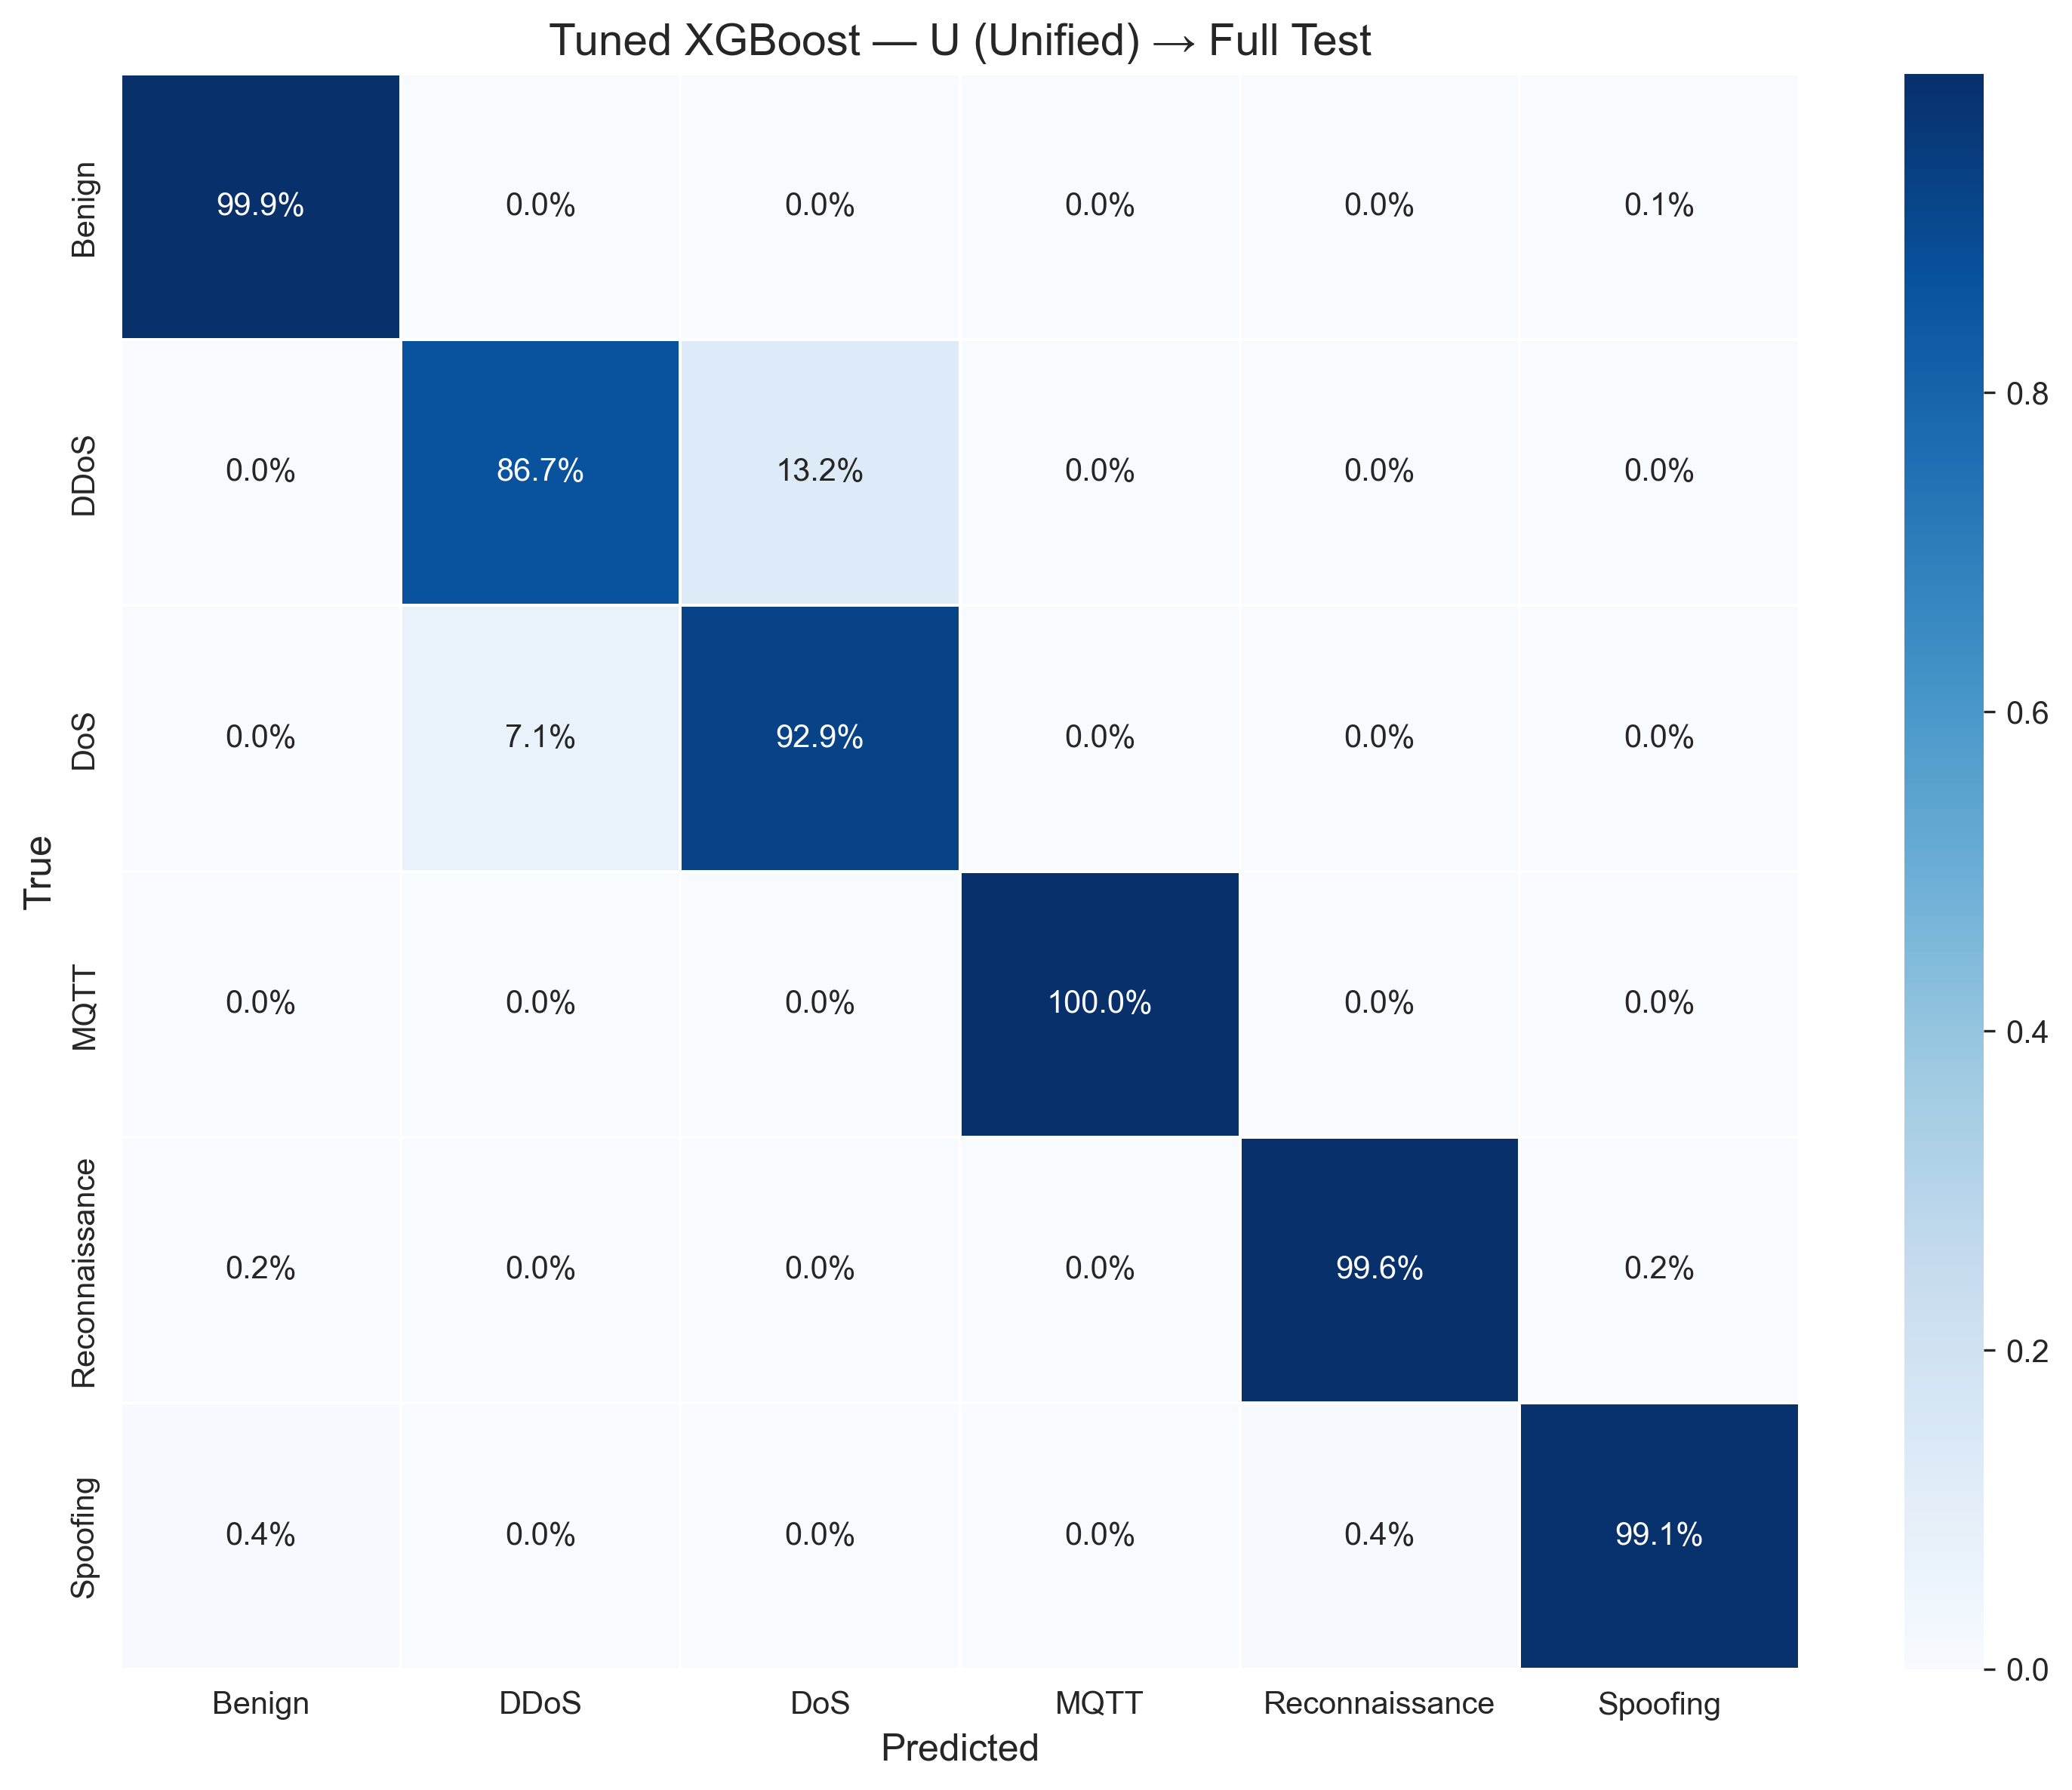
\includegraphics[width=0.62\textwidth]{ch5_xgb_cm_u_full.png}
\caption[]{Κανονικοποιημένος πίνακας σύγχυσης του ρυθμισμένου μοντέλου XGBoost (ενοποιημένο καθεστώς) στο πλήρες σύνολο ελέγχου (1.201.731 δείγματα). Τα σφάλματα συγκεντρώνονται σχεδόν αποκλειστικά στο ζεύγος DDoS--DoS.}
\label{gr:fig:cm}
\end{figure}

Το Σχήμα~\ref{gr:fig:perclass} συγκρίνει το F1 ανά κλάση για τα τρία καθεστώτα του XGBoost: η εκπαίδευση μίας πηγής καταρρέει στις κλάσεις της άλλης πηγής, ενώ το ενοποιημένο μοντέλο ανακτά και τις έξι κλάσεις.

\begin{figure}[!htbp]
\centering
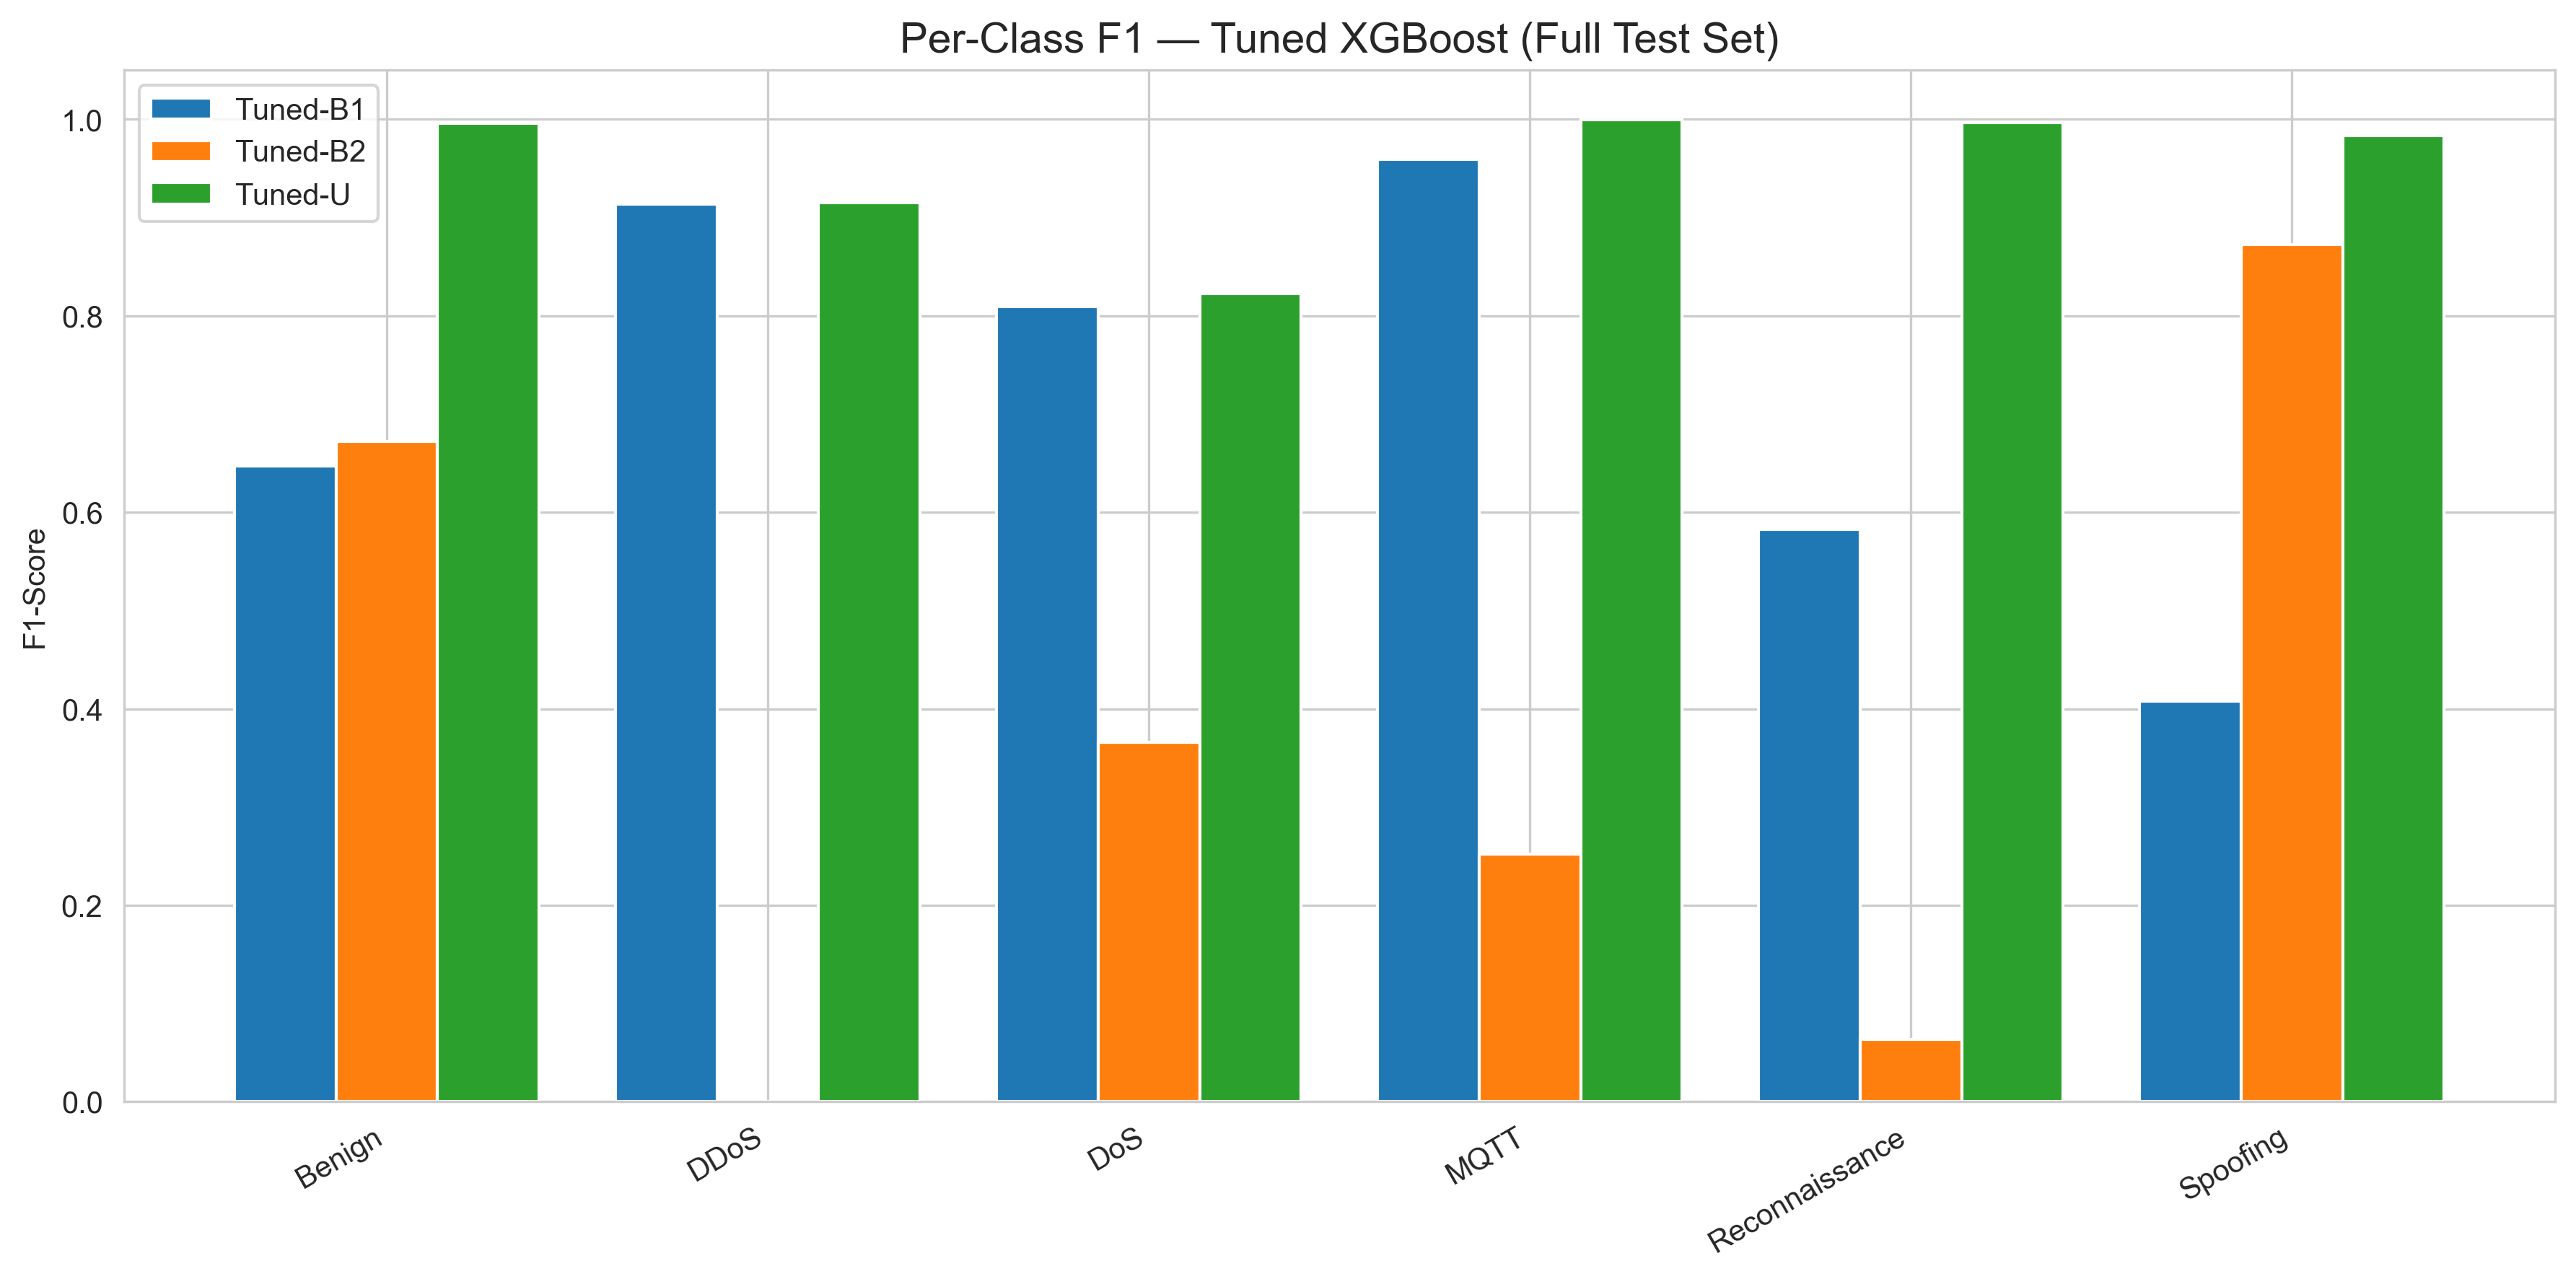
\includegraphics[width=\textwidth]{ch5_xgb_per_class_f1.png}
\caption[]{Σύγκριση του F1 ανά κλάση μεταξύ των καθεστώτων εκπαίδευσης B1, B2 και U (ρυθμισμένο XGBoost, πλήρες σύνολο ελέγχου).}
\label{gr:fig:perclass}
\end{figure}

\grsubsection{Στατιστική σημαντικότητα}

Η σημαντικότητα των διαφορών μεταξύ των ενοποιημένων μοντέλων ελέγχθηκε με τον έλεγχο McNemar~\cite{mcnemar1947note} με διόρθωση συνέχειας Yates, κατάλληλο για ζευγαρωτές παρατηρήσεις στο ίδιο σύνολο ελέγχου. Επειδή με $N = 1.201.731$ δείγματα ακόμη και αμελητέες διαφορές γίνονται στατιστικά σημαντικές, αναφέρεται επιπλέον η σχετική μείωση σφάλματος (RER) ως μέτρο μεγέθους επίδρασης (Πίνακας~\ref{gr:tab:mcnemar}). Το XGBoost υπερέχει στατιστικά και πρακτικά έναντι των DT και RF (RER $\approx$ 3\%, δηλαδή περίπου 4.000 λιγότερα σφάλματα). Η σύγκριση DT--RF είναι στατιστικά σημαντική αλλά πρακτικά οριακή: το RF κάνει ελαφρώς περισσότερα συνολικά σφάλματα, έχει όμως υψηλότερο macro-F1, επειδή μεταφέρει σφάλματα από τις μειοψηφικές κλάσεις προς το όριο DDoS/DoS, που είναι και η επιδιωκόμενη συμπεριφορά της εκπαίδευσης με ισορροπημένα βάρη.

\begin{table}[!htbp]
\centering
\caption[]{Έλεγχος McNemar για τις ζευγαρωτές συγκρίσεις των ενοποιημένων μοντέλων στο πλήρες σύνολο ελέγχου. $b$: το Α σωστό και το Β λάθος· $c$: το Α λάθος και το Β σωστό· RER $> 0$: το Β κάνει λιγότερα σφάλματα.}
\label{gr:tab:mcnemar}
\small
\begin{tabular}{@{}l c c r r r@{}}
\toprule
\textbf{Ζεύγος (Α έναντι Β)} & $b$ & $c$ & $\chi^2$ (Yates) & \textbf{τιμή $p$} & \textbf{RER (\%)} \\
\midrule
DT έναντι RF  & 6.919 & 6.372  & 22,43    & $2{,}2 \times 10^{-6}$ & $-0{,}41$ \\
DT έναντι XGB & 7.314 & 11.297 & 851,99   & $< 10^{-15}$ & $+2{,}98$ \\
RF έναντι XGB & 4.246 & 8.776  & 1.575,17 & $< 10^{-15}$ & $+3{,}38$ \\
\bottomrule
\end{tabular}
\end{table}

% ══════════════════════════════════════════════════════════════════════════════
\grsection{Γενίκευση σε πραγματική νοσοκομειακή κίνηση: HospNet26}

\grsubsection{Σύνολο δεδομένων και πρωτόκολλο}

Το HospNet26~\cite{hospnet26} είναι δημόσιο σύνολο αναφοράς με ανωνυμοποιημένα χαρακτηριστικά κίνησης από το εσωτερικό δίκτυο ενός νοσοκομείου Helios στη Γερμανία, που καταγράφηκε κατά τη διάρκεια μίας εβδομάδας κανονικής κλινικής λειτουργίας (Αύγουστος 2025). Δεν περιέχει ετικέτες επιθέσεων: τεκμηριώνεται ως αποκλειστικά νόμιμη κίνηση και κάθε πρόβλεψη διαφορετική από Benign αποτελεί ψευδώς θετικό. Τα τέσσερα χρονικά τμήματα (Παρασκευή, Σαββατοκύριακο, Δευτέρα, Δευτέρα--Παρασκευή) συνενώθηκαν σε \textbf{1.265.240 παράθυρα}· εξήχθησαν τα 58 χαρακτηριστικά με την ίδια σειρά, εφαρμόστηκε ο \textit{ίδιος} κανονικοποιητής του συνόλου εκπαίδευσης (χωρίς νέα προσαρμογή) και τα τρία ενοποιημένα μοντέλα εφαρμόστηκαν χωρίς επανεκπαίδευση. Ως μετρική χρησιμοποιείται το ποσοστό προβλέψεων Benign $r_B$, το οποίο στη συγκεκριμένη περίπτωση ισούται με την ειδικότητα του μοντέλου.

\grsubsection{Αποτελέσματα}

Όπως δείχνει ο Πίνακας~\ref{gr:tab:hospnet}, και τα τρία μοντέλα ταξινομούν το 90--96\% της πραγματικής νοσοκομειακής κίνησης ως κάποια μορφή επίθεσης, με $r_B$ μόλις 3,72--9,96\%. Η κυρίαρχη κλάση ψευδώς θετικών είναι η DoS (51--72\% των παραθύρων). Το XGBoost επιτυγχάνει το υψηλότερο $r_B$ (9,96\%). Τα παράθυρα του Σαββατοκύριακου εμφανίζουν ακόμη χαμηλότερα ποσοστά Benign (0,86--5,86\%) από τις καθημερινές, γεγονός που υποδηλώνει χρονικά μη στάσιμη μετατόπιση κατανομής. Συμπληρωματικά, στο σχετικό άρθρο δείχνεται ότι και τα μοντέλα μίας πηγής (B1, B2) παραμένουν στην ίδια ζώνη 0--10\%· άρα το χάσμα δεν κλείνει με αλλαγή της σύνθεσης των εργαστηριακών δεδομένων εκπαίδευσης.

\begin{table}[!htbp]
\centering
\caption[]{Κατανομή προβλέψεων των τριών ρυθμισμένων ενοποιημένων μοντέλων σε 1.265.240 παράθυρα πραγματικής νοσοκομειακής κίνησης (HospNet26). Όλη η κίνηση είναι καλόβουλη, επομένως η τελευταία στήλη ($r_B$) είναι η ειδικότητα του μοντέλου και όλες οι υπόλοιπες στήλες είναι ποσοστά ψευδώς θετικών.}
\label{gr:tab:hospnet}
\small
\begin{tabular}{@{}l r r r r r r | r@{}}
\toprule
\textbf{Μοντέλο} & \textbf{Benign} & \textbf{DDoS} & \textbf{DoS} & \textbf{MQTT} & \textbf{Recon.} & \textbf{Spoofing} & \textbf{$r_B$} \\
\midrule
Decision Tree  & 6,07\% &  7,80\% & 72,04\% & 0,22\% &  5,30\% &  8,57\% & \textbf{6,07\%} \\
Random Forest  & 3,72\% &  0,60\% & 71,37\% & 0,06\% & 19,08\% &  5,17\% & \textbf{3,72\%} \\
XGBoost        & 9,96\% & 23,80\% & 51,14\% & 0,11\% &  4,28\% & 10,71\% & \textbf{9,96\%} \\
\bottomrule
\end{tabular}
\end{table}

\grsubsection{Ερμηνεία και στρατηγικές επαναβαθμονόμησης}

Το αποτέλεσμα δεν αποτελεί αποτυχία του μοντέλου, αλλά περίπτωση \textit{μετατόπισης συμμεταβλητών} (covariate shift)~\cite{sommer2010outside}: η κατανομή των καλόβουλων δεδομένων εκπαίδευσης διαφέρει συστηματικά από εκείνη του περιβάλλοντος λειτουργίας. Η καλόβουλη κίνηση των εργαστηριακών συνόλων παρήχθη υπό ελεγχόμενες συνθήκες, ενώ ένα πραγματικό νοσοκομείο μεταφέρει ροές ιατρικής απεικόνισης (DICOM/PACS), συστήματα ηλεκτρονικού φακέλου υγείας (HL7, FHIR), ιδιόκτητα κλινικά πρωτόκολλα και μεγάλο όγκο διοικητικής κίνησης. Οι μεταφορές υψηλού ρυθμού παράγουν στατιστικά τύπου «ριπής» που επικαλύπτονται με την περιοχή χαρακτηριστικών της κλάσης DoS, κάτι που εξηγεί γιατί η DoS κυριαρχεί στα ψευδώς θετικά. Για τη γεφύρωση του χάσματος προτείνονται δύο στρατηγικές χαμηλού κόστους: (α)~\textit{λεπτομερής προσαρμογή με λίγα δείγματα} (few-shot fine-tuning), δηλαδή επανεκπαίδευση με ένα μικρό, επιβεβαιωμένα καλόβουλο δείγμα από το νοσοκομείο-στόχο (περίπου 10.000--50.000 παράθυρα)· και (β)~\textit{εκ των υστέρων βαθμονόμηση κατωφλίου} στις πιθανότητες εξόδου του μοντέλου, με στόχο αποδεκτό ποσοστό ψευδών συναγερμών (π.χ.\ $\leq 1\%$). Και οι δύο απαιτούν μόνο καλόβουλη κίνηση, που είναι άφθονη σε κάθε δίκτυο, και αποφεύγουν τα ηθικά και πρακτικά προβλήματα συλλογής επισημασμένων επιθέσεων σε πραγματικό νοσοκομείο.

% ══════════════════════════════════════════════════════════════════════════════
\grsection{Βιωσιμότητα και ηθικές διαστάσεις}

Από περιβαλλοντική σκοπιά, η εργασία εκτελέστηκε σε συμβατικό υλικό, χωρίς συστοιχίες υψηλών επιδόσεων· η προτίμηση αποδοτικών αλγορίθμων με δέντρα και η δημοσίευση ενός επαναχρησιμοποιήσιμου συνόλου μειώνουν τον υπολογιστικό φόρτο που θα απαιτούσε η επανάληψη της ίδιας προεπεξεργασίας από κάθε ερευνητή. Από οικονομική σκοπιά, όλα τα εργαλεία και τα σύνολα δεδομένων είναι ανοικτά, με ελάχιστο άμεσο κόστος, ενώ το δημόσιο σύνολο (DOI \texttt{10.34810/DATA3305}) αυξάνει τη μακροπρόθεσμη αξία της εργασίας. Κοινωνικά, η εργασία συμβάλλει στην προστασία κρίσιμων υποδομών υγείας και στη διάχυση της γνώσης μέσω αναπαραγώγιμης μεθοδολογίας. Από ηθική σκοπιά, τα σύνολα εκπαίδευσης προέρχονται από ελεγχόμενες πειραματικές διατάξεις χωρίς δεδομένα ασθενών, τα στατιστικά χαρακτηριστικά δεν διατηρούν αναγνωριστικά δικτύου, η εργασία έχει αμιγώς αμυντικό προσανατολισμό και η καταγραφή προέλευσης επιτρέπει τον εντοπισμό μεροληψιών ανά πηγή.

% ══════════════════════════════════════════════════════════════════════════════
\grsection{Συμπεράσματα}

\grsubsection{Απάντηση στο ερευνητικό ερώτημα}

Η απάντηση στο ερευνητικό ερώτημα έχει τρία σκέλη. \textit{Πώς επιτυγχάνεται η ενοποίηση:} με εφαρμογή ενός κοινού εργαλείου εξαγωγής χαρακτηριστικών (MIOTTA-NPT) στις ακατέργαστες καταγραφές κάθε πηγής, εναρμόνιση των ετικετών σε κοινή ταξινομία και συνένωση των εγγραφών με μεταδεδομένα προέλευσης· έτσι αίρονται τα δομικά εμπόδια (Π2, Π3) που αποκλείουν την απλή συνένωση. \textit{Αν βελτιώνει την απόδοση:} ναι· η ενοποιημένη εκπαίδευση αύξησε το macro-F1 στο ετερογενές σύνολο ελέγχου από 0,70--0,74 (καλύτερο μοντέλο μίας πηγής) σε 0,948--0,952, με υψηλή απόδοση και στις έξι κατηγορίες. \textit{Ποια είναι τα όριά της:} η ενοποίηση εργαστηριακών πηγών βελτιώνει τη γενίκευση \textit{μεταξύ αυτών των πηγών}, αλλά δεν κλείνει το χάσμα προς τα πραγματικά κλινικά περιβάλλοντα· η γενίκευση σε επίπεδο λειτουργίας απαιτεί αντιπροσωπευτικά δείγματα από το δίκτυο-στόχο, όπως έδειξε η αξιολόγηση στο HospNet26.

\grsubsection{Περιορισμοί}

Τα ευρήματα πρέπει να ερμηνεύονται λαμβάνοντας υπόψη ότι: (i)~τα δεδομένα εκπαίδευσης προέρχονται από εργαστηριακές διατάξεις· (ii)~ενοποιήθηκαν μόνο δύο πηγές· (iii)~το μέγεθος παραθύρου (100 πακέτα) διατηρήθηκε σταθερό· (iv)~η εναρμόνιση ετικετών περιλαμβάνει υποκειμενικές επιλογές· (v)~το HospNet26 δεν διαθέτει επισημασμένη αλήθεια εδάφους, οπότε κάποια «ψευδώς θετικά» θα μπορούσαν θεωρητικά να είναι πραγματικές επιθέσεις· και (vi)~εξετάστηκαν μόνο μοντέλα βασισμένα σε δέντρα, χωρίς συγκρίσεις με βαθιά μάθηση.

\grsubsection{Μελλοντική εργασία}

Ως άμεση προτεραιότητα προκύπτει η εμπειρική επικύρωση των στρατηγικών επαναβαθμονόμησης με πραγματικά κλινικά δεδομένα και ο προσδιορισμός του απαιτούμενου πλήθους καλόβουλων παραθύρων για αποδεκτή ειδικότητα. Περαιτέρω κατευθύνσεις είναι: η ενσωμάτωση επιπλέον πηγών μέσω της ίδιας αρθρωτής ροής· η χρήση πιο προηγμένης βελτιστοποίησης υπερπαραμέτρων (π.χ.\ Bayesian βελτιστοποίηση με Optuna, Hyperband, BOHB)· η μηχανική χαρακτηριστικών για το όριο DDoS/DoS, όπως η ποικιλομορφία διευθύνσεων πηγής ανά παράθυρο ή η ασυμμετρία όγκου ροών· η διερεύνηση ακολουθιακών μοντέλων βαθιάς μάθησης (1D-CNN, LSTM, Transformer) πάνω στην αναπαράσταση nPrint του MIOTTA-NPT· και, τέλος, η μετάβαση σε πρωτότυπο λειτουργίας πραγματικού χρόνου, με περιορισμούς καθυστέρησης, μνήμης, μετατόπισης εννοιών (concept drift) και κόπωσης από συναγερμούς.

Συνολικά, η εργασία δείχνει ότι η πολυπηγαία ενοποίηση είναι ο καθοριστικός παράγοντας για τη γενίκευση των \gls{ids} μεταξύ εργαστηριακών περιβαλλόντων \gls{iomt}, ενώ η γεφύρωση του χάσματος προς τα πραγματικά κλινικά δίκτυα παραμένει ανοικτή πρόκληση, για την οποία προτείνονται συγκεκριμένες και εφαρμόσιμες λύσεις. Η αποδοχή των ευρημάτων στο SecHealth @ ARES~2026 επιβεβαιώνει ότι η μεθοδολογία και τα αποτελέσματα ανταποκρίνονται στα πρότυπα της διεθνούς ερευνητικής κοινότητας.
